\chapter{Methodology}\label{chap:method}

\section{Tools Used}
Once the preprocessed dataset is obtained, we can enter the implementation level using \acrlong{ML} algorithms. Proceeding to this level, some tools are required that are listed as the following:

\begin{itemize}
    \item \textbf{\acrshort{HUNT} Cloud\footnote{\href{https://www.ntnu.edu/mh/huntcloud/cloud-services/hunt-compute}{https://www.ntnu.edu/mh/huntcloud/cloud-services/hunt-compute}}}: It is a Cloud computing service with Linux-based virtual machines that have varying size and memory capacity. The infrastructure is affiliated to the HUNT Research Centre, Department of Public Health and Nursing, Faculty of Medicine and Health Sciences, \acrfull{NTNU}, in Norway. 
    \item \textbf{Anaconda Spyder}: The platform for our implementations in Python. Albeit there are some other platforms such as Jupyter Lab to run our codes, since we need to have access to variables via \textsl{Variable Explorer}, Anaconda Spyder has a privilege over the other platforms.
    \item \textbf{sklearn}: Scikit-learn is a Python module that provides state-of-the-art implementations of many well-known algorithms in machine learning \cite{pedregosa_scikit-learn_2011}. It has an easy-to-use interface, and it only depends on NumPy and SciPy.
    \item \textbf{xgboost}: Unlike most of the typical \acrshort{ML} algorithms which are included in the sklearn, xgboost must be installed separately. It is an optimized gradient boosting library that solves numerous data science problems quickly and accurately.
    \item \textbf{imblearn}: Python imbalanced learning package is used on datasets where one or more of the classes has significantly less/more training samples. It employs under-sampling or over-sampling techniques to provide an equal ratio of classes.
    \item \textbf{seaborn\footnote{\href{https://seaborn.pydata.org/}{https://seaborn.pydata.org/}}}: Seaborn is a Python data visualization library. It provides a high-level interface for informative statistical graphics and drawing attractive by facilitating data visualization needs.
\end{itemize}

\section{Imbalanced Dataset}
Figure~\ref{fig:aliveexpiredratio} shows the proportion of alive patients over expired ones. It indicates that in our 59190-patient cohort (53\% male), the alive patients dominate the expired patients by a factor of 4.3. Such a significant difference between the members of a binary class affects the final prediction inasmuch as it is expected that the machine estimates most of the outcomes as alive. This prediction is correct, and in most cases, it would have high accuracy, but it could have been achieved even without having expired patients in our class. This is called the \textit{accuracy paradox} and is a common mistake since classification accuracy is the first measure for model evaluation on classification problems.

\begin{figure}[h]
\centering
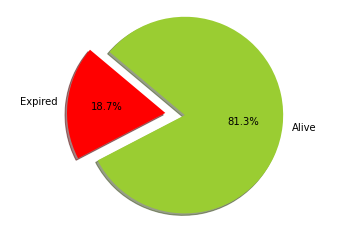
\includegraphics[width=8cm]{fig/chapter4/Alive_vs._Expired_Ratio.png}
\caption{Ratio of the Alive vs. Expired patients}
\label{fig:aliveexpiredratio}
\end{figure}

{\hskip 1em} There are techniques called resampling for balancing the number of class members before implementing the \acrlong{ML} algorithms. If samples are added to the minority class, it would be an over-sampling technique, and if samples are removed from the majority class, it would be an under-sampling technique, as depicted in figure \ref{fig:resampling}. 

\begin{figure}[h]
\centering
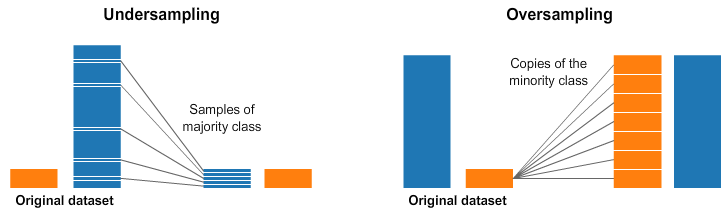
\includegraphics[width=16cm]{fig/chapter4/resampling.png}
\caption{The general concept of the resampling techniques, retrieved from \href{https://www.kaggle.com/rafjaa/resampling-strategies-for-imbalanced-datasets}{\textsl{Kaggle}}}
\label{fig:resampling}
\end{figure}

{\hskip 1em} The simplest over-sampling implementation is by duplicating random records from the minority class, bringing about overfitting. The simplest technique in under-sampling is random records removal from the majority class, giving rise to loss of information.

\subsection{Under-sampling Techniques}
Apart from random under-sampling, there are other techniques to undersample majority class, such as:

\begin{itemize}
    \item \textbf{Cluster Centroids}: It generates clustering-based centroids. Similar data should be grouped previously in order to preserve information.
    \item \textbf{Near Miss}: It comprises three versions, all of which select samples based on the distance between the majority and the minority class.
    \item \textbf{\acrlong{CNN} Rule}: \acrshort{CNN} seeks a subset of samples that leads to no loss in model performance, considered as a minimal consistent set.
    \item \textbf{Tomek Links}: It consists of removing the majority class's instances close to the minority class to space up the distance in-between; hence, facilitating the classification process.
    \item \textbf{\acrlong{ENN} Rule}: \acrshort{ENN} uses three nearest neighbors to locate misclassified samples and then uses the nearest one to make decisions.
    \item \textbf{\acrlong{OSS}}: \acrshort{OSS} is a combination of Tomek Links and \acrlong{CNN}. It involves removing the ambiguous samples on the class boundary from the majority class (Tomek Links) and then removing the redundant samples of the majority class that are far from the decision boundary (\acrshort{CNN}).
    \item \textbf{\acrlong{NCR}}: \acrshort{NCR} combines \acrshort{CNN} to remove redundant samples and \acrshort{ENN} to remove noisy or ambiguous samples.
\end{itemize}

{\hskip 1em} Concerning all the techniques mentioned above, since we lost a bunch of data due to the lactate sample limitation, we are more interested in utilizing over-sampling methods.

\subsection{Over-sampling Techniques}
There are different oversampling techniques to be applied to an imbalanced dataset. Some of their typical ones are as follows:

\begin{itemize}
    \item \textbf{Na\"ive Random Oversampling}: From the under-represented class, it generates new samples by randomly sampling with replacement of the currently available samples.
    \item \textbf{\acrlong{SMOTE}}: \acrshort{SMOTE} works by creating synthetic elements from the minor class instead of creating copies. The algorithm works by randomly selecting a point from the minority class and computing the k-nearest neighbors. The synthetic points are then added between the chosen point and its neighbors.
    \item \textbf{\acrlong{ADASYN} Sampling Method}: Derived from \acrshort{SMOTE}, \acrshort{ADASYN} has only one important difference. It biases the sample space toward the minority class.
    \item \textbf{Other Combinations}: There are other \acrshort{SMOTE}-derived techniques such as SMOTE-Boost, BorderlineSMOTE, SVMSMOTE, KMeansSMOTE, and SMOTENC that defined for particular purposes like dealing with categorical features.
\end{itemize}

{\hskip 1em} It is also possible to use an over-sampling technique followed by an under-sampling method, which yields impressive results. Whilst an over-sampling can improve the bias toward the minority class, an under-sampling can reduce the bias on the majority class. This can result in enhanced overall performance. \

{\hskip 1em} Contemplating all the aforementioned techniques and our imbalanced dataset, we chose \acrfull{SMOTE} to balance the cohort before entering the \acrlong{ML} stage. By using \acrshort{SMOTE}, as illustrated in figure \ref{fig:smote} (particularly \ref{fig:aftersmote} \& \ref{fig:balanced}), it can be seen that our dataset is balanced now and ready for further \acrshort{ML} analysis.

\begin{figure}[H]
\begin{tabular}{@{}cc@{}}
\begin{subfigure}{0.5\textwidth}
  \centering
  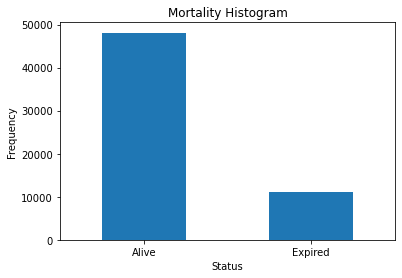
\includegraphics[width=7.5cm]{fig/chapter4/Before SMOTE.png}
  \caption{\footnotesize{Actual patients frequency}}
  \label{fig:beforesmote}
\end{subfigure} 
\begin{subfigure}{0.5\textwidth}
  \centering
  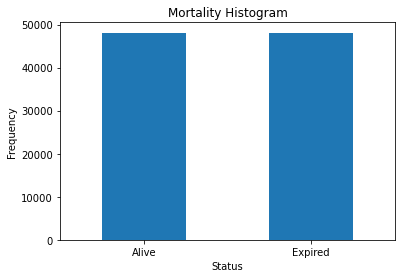
\includegraphics[width=7.5cm]{fig/chapter4/After SMOTE.png}
  \caption{\footnotesize{Patients frequency after applying \acrshort{SMOTE}}}
  \label{fig:aftersmote}
\end{subfigure} \\
\begin{subfigure}{0.5\textwidth}
  \centering
  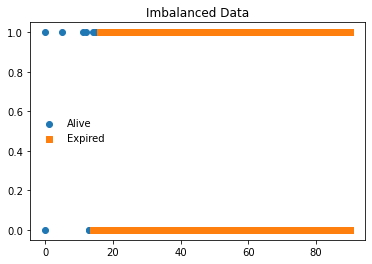
\includegraphics[width=7.5cm]{fig/chapter4/Imbalanced Data.png}
  \caption{\footnotesize{The cohort's actual scattering plot}}
  \label{fig:imbalanced}
\end{subfigure} 
\begin{subfigure}{0.5\textwidth}
  \centering
  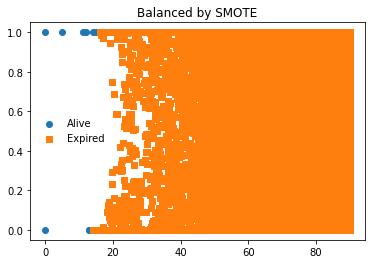
\includegraphics[width=7.5cm]{fig/chapter4/SMOTE Scattering Plot.png}
  \caption{\footnotesize{The cohort's scattering plot after applying \acrshort{SMOTE}}}
  \label{fig:balanced}
\end{subfigure} \\
\end{tabular}
\caption{Utilization of \acrshort{SMOTE} to balance an imbalanced dataset}
\label{fig:smote}
\end{figure}

\section{Glucose vs. Lactate}
Despite the fact that our primary goal is to predict mortality using various features, including glucose and lactate, it would be interesting to set a secondary goal on checking if glucose and lactate themselves are related mathematically or not. From \cite{greco_diabetes_2018}, we know that both are interdependent in carbohydrate metabolism, but as engineers, we need to find out more; perhaps, correlation can elucidate more details in this regard. Figure \ref{fig:heatmap} delineates the correlation between all the input variables of the cohort. It shows that excluding a modest association of glucose with \acrshort{DM}, which Greco et al. mentioned in \cite{greco_diabetes_2018}, there is almost no relationship between our dataset's input parameters. To make sure of this, we plotted the scattering distribution of lactate and glucose among the dataset patients based on their outcome, as shown in figure \ref{fig:gluclact}. The distribution in figures \ref{fig:gluclactmin} and \ref{fig:gluclactmean} are dense while it is widespread in figure \ref{fig:gluclactmax}. Nevertheless, in none of which, there is a clue of classification between glucose and lactate.

\begin{figure}[ht]
\centering
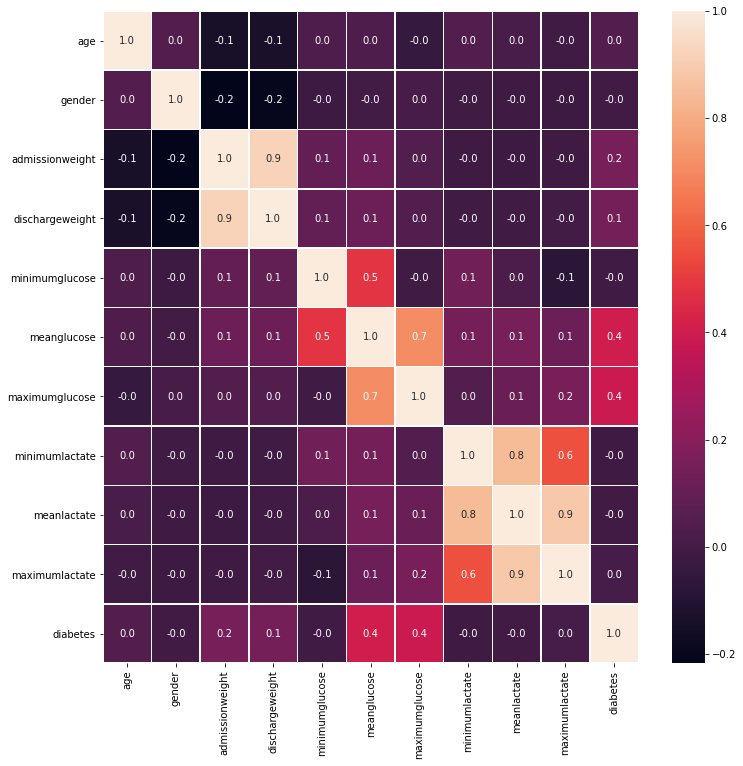
\includegraphics[width=16cm]{fig/chapter4/Heatmap.png}
\caption{The correlation matrix of the dataset}
\label{fig:heatmap}
\end{figure}

{\hskip 1em} Eventually, we take one last step and apply the pairs plot (aka scatterplot matrix) to see every variable's distribution and relationships between two variables. Looking at figure \ref{fig:pairplot}, we can rest assured that finding a mathematical relationship between glucose and lactate is way complicated.

\begin{figure}[H]
\begin{tabular}{@{}c@{}}
\begin{subfigure}{1\textwidth}
  \centering
  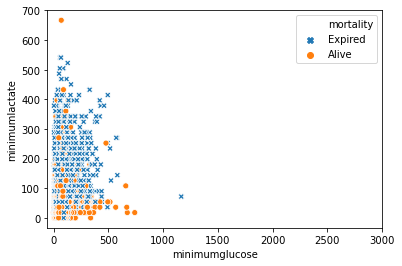
\includegraphics[width=10cm]{fig/chapter4/Glu-Lac, Min.png}
  \caption{\footnotesize{The scattering plot for the minimum values of glucose and lactate}}
  \label{fig:gluclactmin}
\end{subfigure} \\
\begin{subfigure}{1\textwidth}
  \centering
  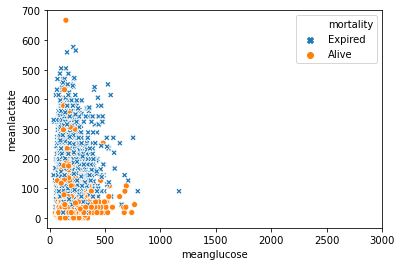
\includegraphics[width=10cm]{fig/chapter4/Glu-Lac, Mean.png}
  \caption{\footnotesize{The scattering plot for the mean values of glucose and lactate}}
  \label{fig:gluclactmean}
\end{subfigure} \\
\begin{subfigure}{1\textwidth}
  \centering
  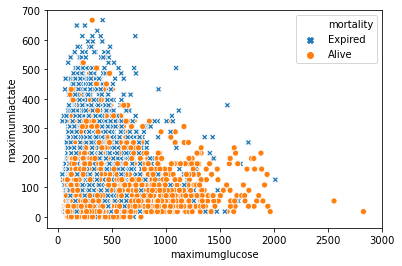
\includegraphics[width=10cm]{fig/chapter4/Glu-Lac, Max.png}
  \caption{\footnotesize{The scattering plot for the maximum values of glucose and lactate}}
  \label{fig:gluclactmax}
\end{subfigure} \\
\end{tabular}
\caption{The scattering plot of lactate vs. glucose for three different levels}
\label{fig:gluclact}
\end{figure}

\begin{figure}[ht]
\centering
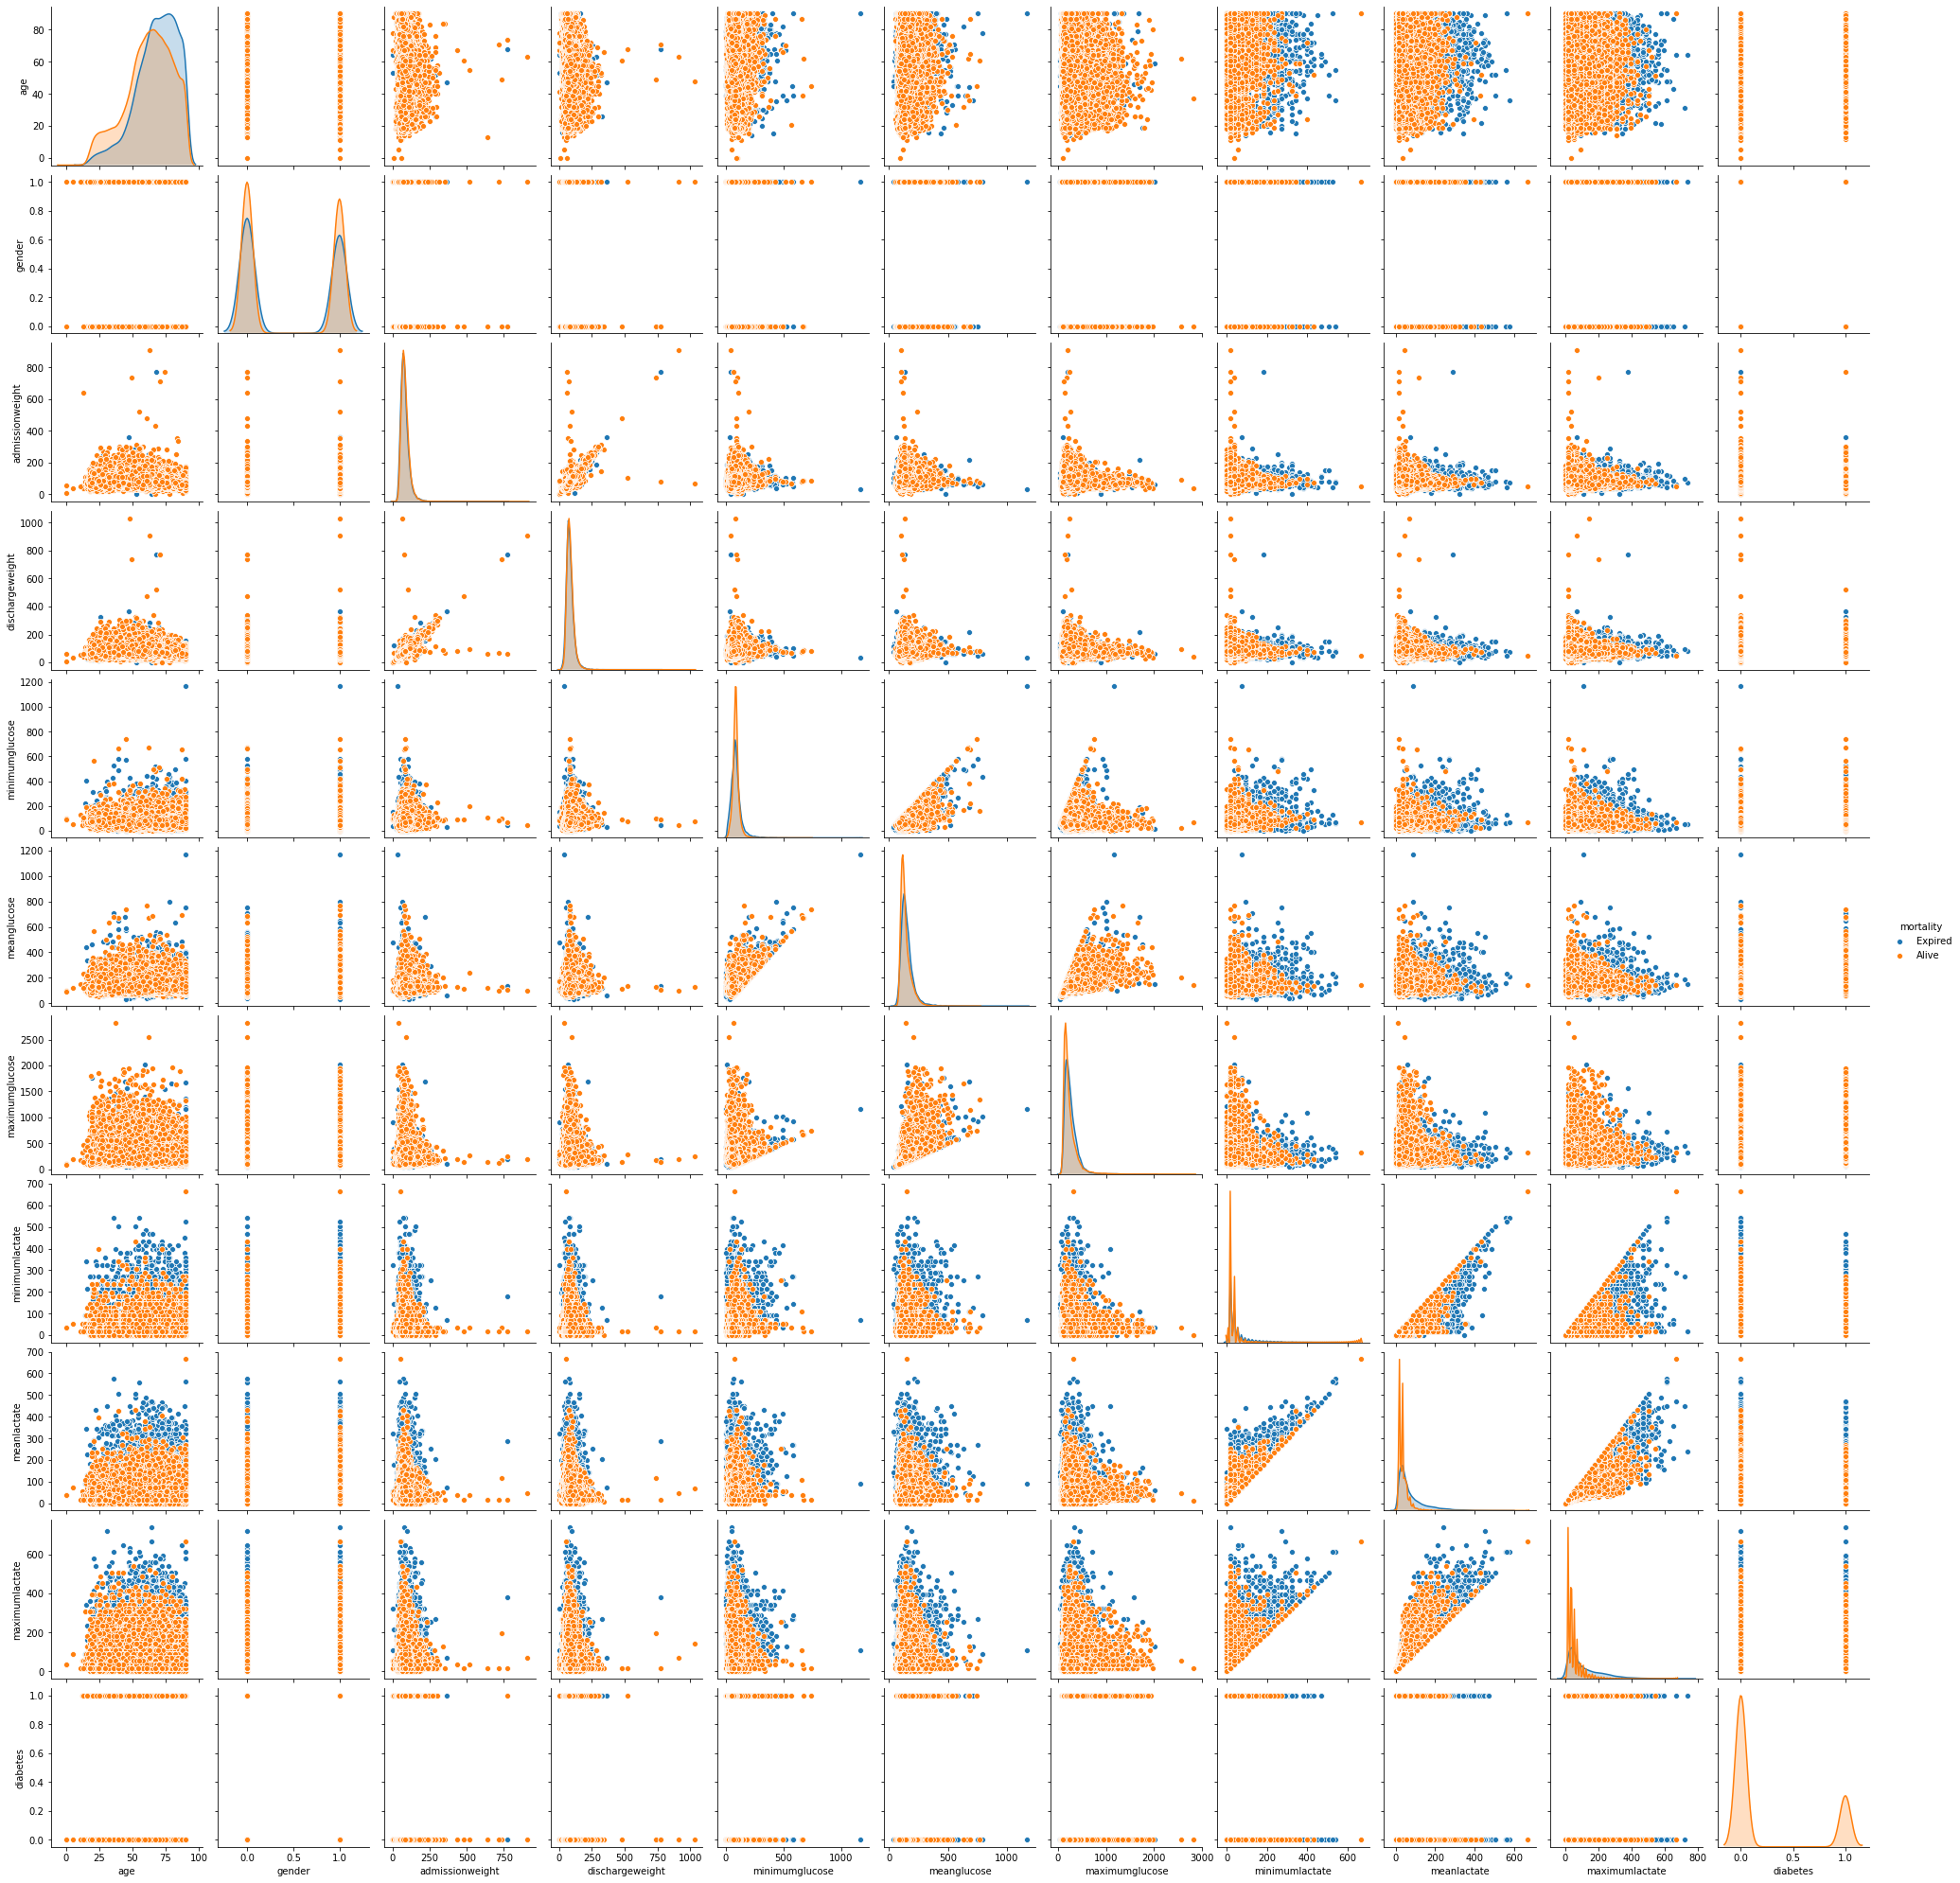
\includegraphics[width=16cm]{fig/chapter4/PairPlot.png}
\caption{The scatterplot matrix of the dataset's input features}
\label{fig:pairplot}
\end{figure}

\section{Implementation}
Seven typical linear and non-linear \acrlong{ML} algorithms have been implemented to analyze the cohort. All of them are discussed in this section. The results are given in chapter \ref{chap:results}, however. \

{\hskip 1em} Before entering the implementation level, note that 25\% of the initial cohort is split off to form a validation cohort, leaving 44,392 patients for model training if \acrshort{SMOTE} is not used and 72,144 patients if \acrshort{SMOTE} is applied. The dataset has 11 columns as input features (see figure \ref{fig:cohortselection}) and \textsl{mortality} as the binary class output feature. Moreover, the hyperparameters of all the models are selected by ten-fold cross-validation.

\subsection{Classification And Regression Tree}
Decision Tree is a supervised \acrlong{ML} algorithm used for predictive modeling. The classical \acrfull{CART} provides a basis for some useful algorithms like bagged decision trees, random forest, and boosted decision trees \cite{brownlee_master_2016}. Its representation is binary to make predictions straightforward. Each tree's root node represents an input variable, while each leaf node includes an output variable. Each new input traverses the tree starting from the root node to be evaluated. The algorithm stops splitting when a count on the number of training instances is less than a minimum threshold. \\

\begin{table}[h]
\centering
\setlength\tabcolsep{100pt}
\caption{\label{tab:carthyperparam}\acrshort{CART} basic hyperparameters}
\begin{tabular}{@{}cc@{}}
\toprule
\thead{Hyperparameter}          & \thead{Value}         \\ \midrule \midrule
Learning rate                   & 0.4                   \\ \midrule
Number of trees                 & 1                     \\ \midrule
Maximum tree depth              & 128                   \\
\bottomrule
\end{tabular}
\end{table}

{\hskip 1em} Table \ref{tab:carthyperparam} summarizes a subset of hyperparameters for the \acrshort{CART} model, while figure \ref{fig:cartfeatureimp} shows the algorithm's attributes importance. The importance default type is \textsl{gain} that indicates the average gain across all splits the feature is used in. There are also other types of feature importance, such as \textsl{weight}, \textsl{cover}, \textsl{total gain}, and \textsl{total cover}. It should be mentioned that feature importance is only defined for tree boosters.

\begin{figure}[ht]
\centering
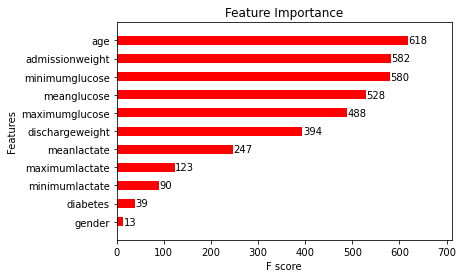
\includegraphics[width=14cm]{fig/chapter4/Feature Importance_CART.png}
\caption{\acrshort{CART} feature importance}
\label{fig:cartfeatureimp}
\end{figure}

\subsection{Extreme Gradient Boosting Decision Tree}
\acrfull{XGB} is an improved version of a Decision-Tree-based ensemble \acrlong{ML} algorithm that uses a gradient boosting framework. It is designed to enhance existing boosting techniques in the shortest amount of time by its hardware and software capabilities \cite{malik_xgboost_2020}. Unlike artificial neural networks, which are superior in unstructured data problems, for small- or medium-size tabular data problems, Decision-Tree-based algorithms are the best-in-class for now. Figure \ref{fig:xgbevolution} elaborates on the evolution of \acrshort{XGB} from Decision Trees.

\begin{figure}[ht]
\centering
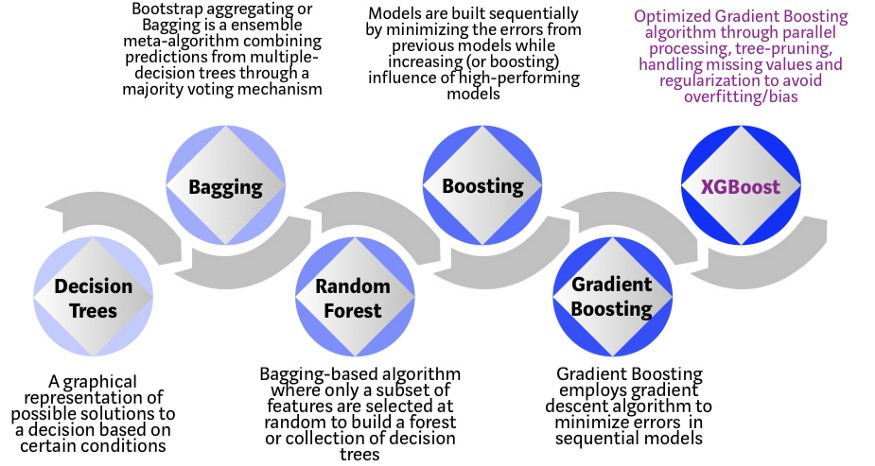
\includegraphics[width=16cm]{fig/chapter4/XGBEvolution.jpeg}
\caption{\acrshort{XGB} algorithm evolution, retrieved from \href{https://towardsdatascience.com/https-medium-com-vishalmorde-xgboost-algorithm-long-she-may-rein-edd9f99be63d}{\textsl{Towards Data Science}}}
\label{fig:xgbevolution}
\end{figure}

{\hskip 1em} Figure \ref{fig:xgbfeatures} illustrates the advantages of the \acrshort{XGB} that makes it a winning \acrlong{ML} algorithm. From parallelizing the generating trees sequential process that reduces the implementation running time to having a built-in grid search to optimize the parameters, all imply the \acrshort{XGB} is a powerful tool for our goal.

{\hskip 1em} The \acrshort{XGB} also has a built-in function to plot features ordered by their importance \cite{malik_xgboost_2020}, the same as in \acrshort{CART}. Figure \ref{fig:xgbfeatureimportance} represents the most important input features for our \acrshort{XGB} algorithm in decreasing order. Furthermore, table \ref{tab:xgbhyperparam} describes the basic hyperparameters used in our implementation.

{\hskip 1em} There is a relationship between the \textsl{Number of trees} and the depth of each tree in table \ref{tab:xgbhyperparam}. We expect that the deeper the trees are, the fewer trees are required in the model, and vice versa. That is to say, the simpler trees need more trees to achieve similar results.


\begin{figure}[ht]
\centering
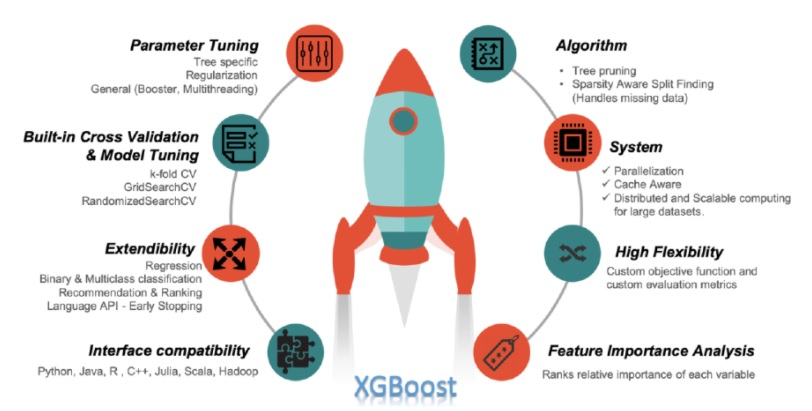
\includegraphics[width=12.7cm]{fig/chapter4/XGB Features.jpg}
\caption{\acrshort{XGB} features \cite{malik_xgboost_2020}}
\label{fig:xgbfeatures}
\end{figure}

\begin{table}[H]
\centering
\setlength\tabcolsep{100pt}
\caption{\label{tab:xgbhyperparam}\acrshort{XGB} basic hyperparameters}
\begin{tabular}{@{}cc@{}}
\toprule
\thead{Hyperparameter}          & \thead{Value}         \\ \midrule \midrule
Learning rate                   & 0.2                   \\ \midrule
Number of trees                 & 100                   \\ \midrule
Maximum tree depth              & 64                    \\
\bottomrule
\end{tabular}
\end{table}

\begin{figure}[H]
\centering
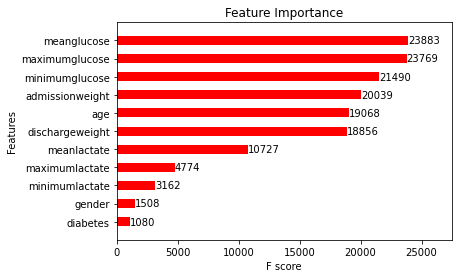
\includegraphics[width=14cm]{fig/chapter4/Feature Importance_XGB.png}
\caption{\acrshort{XGB} feature importance}
\label{fig:xgbfeatureimportance}
\end{figure}

\subsection{Support Vector Machine}
The \acrfull{SVM} algorithm finds a hyperplane decision boundary in an N-dimensional (N-feature) space that best classifies the data points into two classes. This hyperplane should have the maximum distance between the data points of both classes. Support vectors are data points closer to the hyperplane and influence the position and orientation of it.

{\hskip 1em} The \acrlong{SVM} algorithm is mostly effective for balanced datasets and binary classification. For our imbalanced cohort, \acrshort{SVM} should weigh the margin proportional to the class importance, which is often referred to as weighted \acrshort{SVM}, or cost-sensitive \acrshort{SVM} \cite{brownlee_master_2016}. The reason why we choose \textsl{Class weight} parameter as BALANCED, as shown in Table \ref{tab:svmhyperparam}, is due to using \acrshort{SMOTE} beforehand to level the two classes. Furthermore, keep in mind that setting \textsl{Probability} to TRUE slows down the method since it uses five-fold cross-validation\footnote{\href{https://scikit-learn.org/stable/modules/generated/sklearn.svm.SVC.html}{https://scikit-learn.org/stable/modules/generated/sklearn.svm.SVC.html}} internally.

\begin{table}[H]
\centering
\setlength\tabcolsep{100pt}
\caption{\label{tab:svmhyperparam}\acrshort{SVM} basic hyperparameters}
\begin{tabular}{@{}cc@{}}
\toprule
\thead{Hyperparameter}     & \thead{Value}           \\ \midrule \midrule
Kernel                     & radial basis function   \\ \midrule
Gamma                      & scale                   \\ \midrule
Class weight               & balanced                \\ \midrule
Probability                & true                    \\
\bottomrule
\end{tabular}
\end{table}

\subsection{Logistic Regression}
Like \acrshort{SVM}, \acrfull{LR} works well on binary classification, but it is not effective at imbalanced classification. \acrshort{LR} uses an optimization algorithm to minimize the negative-log likelihood (loss) on the training set. Regardless of \acrshort{SMOTE} that we used in our implementation, it is feasible to modify the loss calculation by weighing each class's importance to take the balance into consideration. This can be done by penalizing the model less/more for errors made on majority/minority class samples. This is referred to as Weighted Logistic Regression, Class-Weighted Logistic Regression, or Cost-Sensitive Logistic Regression \cite{brownlee_master_2016}. 

\begin{table}[H]
\centering
\setlength\tabcolsep{100pt}
\caption{\label{tab:lrhyperparam}\acrlong{LR} basic hyperparameters}
\begin{tabular}{@{}cc@{}}
\toprule
\thead{Hyperparameter}     & \thead{Value}           \\ \midrule \midrule
Solver                     & Newton                  \\ \midrule
Penalty                    & L2                      \\ \midrule
Class weight               & balanced                \\
\bottomrule
\end{tabular}
\end{table}

{\hskip 1em} Table \ref{tab:lrhyperparam} shows some of the basic hyperparameters used in our implementation. NEWTON's method is chosen as the model \textsl{Solver} since it uses a better quadratic function minimization. However, the LIBLINEAR method could also be used. Moreover, our algorithm's regularization technique is Ridge Regression (L2), which adds “squared magnitude” of coefficient as a penalty term to the loss function\footnote{\href{https://towardsdatascience.com/l1-and-l2-regularization-methods-ce25e7fc831c}{https://towardsdatascience.com/l1-and-l2-regularization-methods-ce25e7fc831c}}. Finally, applying \acrshort{SMOTE} makes us select the \textsl{Class weight} as BALANCED, the same as in \acrshort{SVM}.

\subsection{Na\"ive Bayes}
The Bayes Theorem assumes each input variable is dependent upon other variables. This brings about calculation complexity. By assuming independence between the variables, the calculation is simplified dramatically. This simplification is widely used for classification problems of predictive modeling and is referred to as \acrfull{NB} \cite{brownlee_master_2016}. 

There are three common distributions in the \acrlong{NB} implementation:

\begin{itemize}
    \item Bernoulli distribution
    \item Gaussian distribution
    \item Multinomial distribution
\end{itemize}

{\hskip 1em} Each of them has its own \acrlong{NB} algorithm. For our case, it is possible to use either Bernoulli \acrlong{NB} or Gaussian \acrlong{NB} algorithm. We go for the latter one, considering the parameter \textsl{priors} should be set appropriately for our imbalanced dataset.

\subsection{Linear Discriminant Analysis}
Limitations such as having a problem with multi-class classification, instability with well-separated classes, and instability with few examples diminish the \acrlong{LR} efficacy in classification problems. Nonetheless, a good alternative is using \acrfull{LDA}. 

{\hskip 1em} Making predictions in \acrshort{LDA} is preceded by computing the statistical properties of the data. It means for a single input variable, the mean and the variance of each class should be extracted, while for multiple variables, this should be done for the means and the covariance matrix \cite{brownlee_master_2016}. Afterwards, Bayes Theorem is used to estimate the probabilities in order to make predictions. 

{\hskip 1em} Table \ref{tab:ldahyperparam} represents the basic parameters used in our project's \acrshort{LDA} algorithm implementation. As can be seen, the \textsl{Solver} is chosen as \acrfull{SVD} with the chance of computing the weighted covariance matrix. The \textsl{Priors} is set to 0.5 for each class, and the \textsl{Number of components} is ONE since it must be the minimum of the number of features or the number of classes subtracted by one\footnote{\href{https://scikit-learn.org/stable/modules/generated/sklearn.discriminant_analysis.LinearDiscriminantAnalysis.html}{https://scikit-learn.org/stable/modules/generated/sklearn.discriminant\_analysis.LinearDiscriminantAnalysis}}. 

\begin{table}[H]
\centering
\setlength\tabcolsep{100pt}
\caption{\label{tab:ldahyperparam}\acrshort{LDA} basic hyperparameters}
\begin{tabular}{@{}cc@{}}
\toprule
\thead{Hyperparameter}     & \thead{Value}           \\ \midrule \midrule
Solver                     & svd                     \\ \midrule
Store covariance           & true                    \\ \midrule
Priors                     & 0.5                     \\ \midrule
Number of components       & 1                       \\
\bottomrule
\end{tabular}
\end{table}

\subsection{K-Nearest Neighbors}
\acrfull{KNN} directly uses the training set to make predictions by searching through it for the K most similar instances and summarizing the output variable, the most common class value, for them. In this regard, a distance measure (e.g., Euclidean distance, Hamming distance, Manhattan distance, Minkowski distance) should be used.

{\hskip 1em} \acrshort{KNN} is well-suited for a small number of input variables. However, for considerably large input variables, it suffers from "Curse of Dimensionality." Therefore, \acrshort{KNN} works fine if the data is low-dimensional, rescaled, and missed data is addressed \cite{brownlee_master_2016}.

{\hskip 1em} In table \ref{tab:knnhyperparam}, some basic parameters for \acrshort{KNN} model implementation are shown. Taking the \textsl{Number of neighbors} as 25, and the \textsl{Metric} as EUCLIDEAN distance gives our study the most accurate result. Besides, the \textsl{Power parameter} is set to 2 (L2), which corresponds to the selected metric.

{\hskip 1em} Apart from built-in feature importance (previously seen in \acrshort{CART} and \acrshort{XGB} sections) and SHAP model-agnostic feature importance (based on the Shapley values from game theory), there is also permutation-based feature importance that shuffles the features and calculates the change in the performance of the model\footnote{\href{https://mljar.com/blog/feature-importance-xgboost/}{https://mljar.com/blog/feature-importance-xgboost/}}. Using this method, we can see the most important features of the \acrshort{KNN}, as depicted in figure \ref{fig:knnfeatureimportance}.

\begin{table}[H]
\centering
\setlength\tabcolsep{100pt}
\caption{\label{tab:knnhyperparam}\acrlong{KNN} basic hyperparameters}
\begin{tabular}{@{}cc@{}}
\toprule
\thead{Hyperparameter}     & \thead{Value}          \\ \midrule \midrule
Number of neighbors        & 25                     \\ \midrule
Algorithm                  & auto                   \\ \midrule
Metric                     & Euclidean              \\ \midrule
Power parameter            & 2                      \\
\bottomrule
\end{tabular}
\end{table}

\begin{figure}[H]
\centering
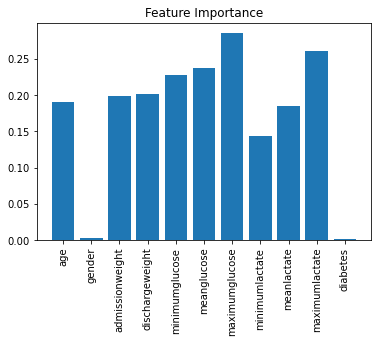
\includegraphics[width=11cm]{fig/chapter4/Feature Importance_KNN.png}
\caption{\acrlong{KNN} feature importance}
\label{fig:knnfeatureimportance}
\end{figure}